\documentclass[10pt,a4paper]{article}
\usepackage[latin1]{inputenc}
\usepackage{amsmath}
\usepackage{amsfonts}
\usepackage{amssymb}
\usepackage{graphicx}
\author{Alexander Bruns}
\title{Multiple Regression on the mtcars dataset}
\begin{document}
	\part{Multiple Regression on the mtcars dataset}
	\textit{Alexander Bruns}
	\section{Summary}
	This study reviews the effect of 10 parameters on the gas mileage of 32 cars. The impact of each factor was investigated and modeled. 
	It was found that the transmission type has no significant effect on the gas mileage. There are gasoline saving autmomatic automobiles availible as well as gasoline saving manual automobile.
	However, these findings only apply to this dataset, because it consists of very few  observations and besides some exotic cars high hp cars are included; thus they do not represent the average car market.
	\subsection{Effect of transmission type on mpg based on the \textit{mtcars} dataset}
	
	The present study aims to investigate the possible effect of the transmission type in 32 cars represented in the \textit{mtcars} dataset among other variables.
	
	This report is divided into three parts: Exploratory data analysis, Model selection and Model validation.
	
	\subsection{Exploratory Data Analysis}
	
	The exploratory data analysis (Appendix A) showed a strong correlation between mpg and weight, displacement and cylinders (R $>$ 0.8). Displacement and cylinders are confounded as usually the displacement increases with cylinder number. Both are correlated with R $>$ 0.9. The correlation between \textit{mpg} and transmission type \textit{am} is about 0.6 which indicates that mpg depends on various factors and not only the transmission type. 
	
	Graph 1 reveals the relation between Weight, Transmission type and Miles per Gallon
	
	\begin{figure}
\centering
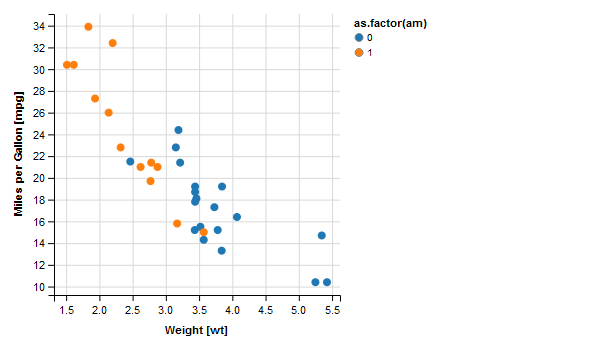
\includegraphics{Rplot}
\caption[mpg vs weight and transmission type (0 - automatic, 1 - manual)]{mpg vs weight and transmission type (0 - automatic, 1 - manual}

\end{figure}
	
\subsection{Model Selection}

This section describes the selection of the best model for the question to how extent affects the transmission type the \textit{mpg}. As shown in the previous section, only the variables with the highest correlation coefficient were taken into account. The selection of the best model is done by means of a likelihood-ratio-test.

\begin{verbatim}
Analysis of Variance Table

Model 1: mpg ~ cyl + disp + hp + drat + wt + qsec + vs + am + gear + carb
Model 2: mpg ~ wt + am + cyl
Model 3: mpg ~ wt + am + cyl + wt * cyl
Res.Df    RSS Df Sum of Sq      F  Pr(>F)  
1     21 147.49                              
2     28 191.05 -7   -43.553 0.8858 0.53445  
3     27 154.31  1    36.736 5.2304 0.03268 *
---
Signif. codes:  0 ?***? 0.001 ?**? 0.01 ?*? 0.05 ?.? 0.1 ? ? 1
\end{verbatim}
The result of the ANOVA table shows that the addition of an interaction term increases the accuray. Therefore the linear model \textit{fit\_interact} will be used the calculate prediction and confidence intervals.

\subsection{Model Evaluation}
The following table shows the summary of the linear model. As it can be seen, the transmission type has no significant effect on mpg. Weight [wt] and cylinders [cyl] are significant regressors. 
In fact, the gas mileage \textbf{does not} depent on the transmission type.
		
\begin{verbatim}
Call:
lm(formula = mpg ~ wt + am + cyl + wt * cyl, data = mtcars)

Residuals:
Min      1Q  Median      3Q     Max 
-4.7887 -1.3812 -0.5268  1.3155  5.3945 

Coefficients:
Estimate Std. Error t value Pr(>|t|)    
(Intercept)  57.0173     7.3507   7.757 2.43e-08 ***
wt           -9.5003     2.6492  -3.586 0.001308 ** 
am           -0.8619     1.2622  -0.683 0.500524    
cyl          -4.0111     1.0594  -3.786 0.000777 ***
wt:cyl        0.8858     0.3494   2.535 0.017337 *  
---
Signif. codes:  0 ?***? 0.001 ?**? 0.01 ?*? 0.05 ?.? 0.1 ? ? 1

Residual standard error: 2.391 on 27 degrees of freedom
Multiple R-squared:  0.863,	Adjusted R-squared:  0.8427 
F-statistic: 42.51 on 4 and 27 DF,  p-value: 2.815e-11
\end{verbatim}		
Residuals (see \textbf{Annex C}) are in a good approximation normally distributed. No autocorrelation nor heteroskedasticity could be observed.
However, two car models - the Toyota Corolla and the Fiat 128 - show greater residuals tha expectetd. This might be due to the fact that these small cars were engineered to save gasoline, opposite to the majority of the investigated population.
\newpage
\appendix
\section{APPENDIX -  Getting and Cleaning the mtcars Data}
\textbf{Requiered packages:}
\begin{itemize}
	\item lattice
	\item psych
	\item ggplot
	\item datasets
\end{itemize}

\section{Inspection for relationship between dependent and independent variables}

The dependent variable is \textit{mpg} while the independent variables are weight \textit{wt}, transmission type \textit{am}, cylinder displacement \textit{disp} and horsepower \textit{hp}. 

Firstly, the correlations between all variables are investigated.

\begin{verbatim}
Call:corr.test(x = mtcars)
Correlation matrix 
mpg   cyl  disp    hp  drat    wt  qsec    vs    am  gear  carb
mpg   1.00 -0.85 -0.85 -0.78  0.68 -0.87  0.42  0.66  0.60  0.48 -0.55
cyl  -0.85  1.00  0.90  0.83 -0.70  0.78 -0.59 -0.81 -0.52 -0.49  0.53
disp -0.85  0.90  1.00  0.79 -0.71  0.89 -0.43 -0.71 -0.59 -0.56  0.39
hp   -0.78  0.83  0.79  1.00 -0.45  0.66 -0.71 -0.72 -0.24 -0.13  0.75
drat  0.68 -0.70 -0.71 -0.45  1.00 -0.71  0.09  0.44  0.71  0.70 -0.09
wt   -0.87  0.78  0.89  0.66 -0.71  1.00 -0.17 -0.55 -0.69 -0.58  0.43
qsec  0.42 -0.59 -0.43 -0.71  0.09 -0.17  1.00  0.74 -0.23 -0.21 -0.66
vs    0.66 -0.81 -0.71 -0.72  0.44 -0.55  0.74  1.00  0.17  0.21 -0.57
am    0.60 -0.52 -0.59 -0.24  0.71 -0.69 -0.23  0.17  1.00  0.79  0.06
gear  0.48 -0.49 -0.56 -0.13  0.70 -0.58 -0.21  0.21  0.79  1.00  0.27
carb -0.55  0.53  0.39  0.75 -0.09  0.43 -0.66 -0.57  0.06  0.27  1.00
Sample Size 32
\end{verbatim}
Then, all variables with a correlation with *mpg* higher than 0.6 are visualized in the following plot in order to examine the type of the correlation.

\begin{figure}
\centering
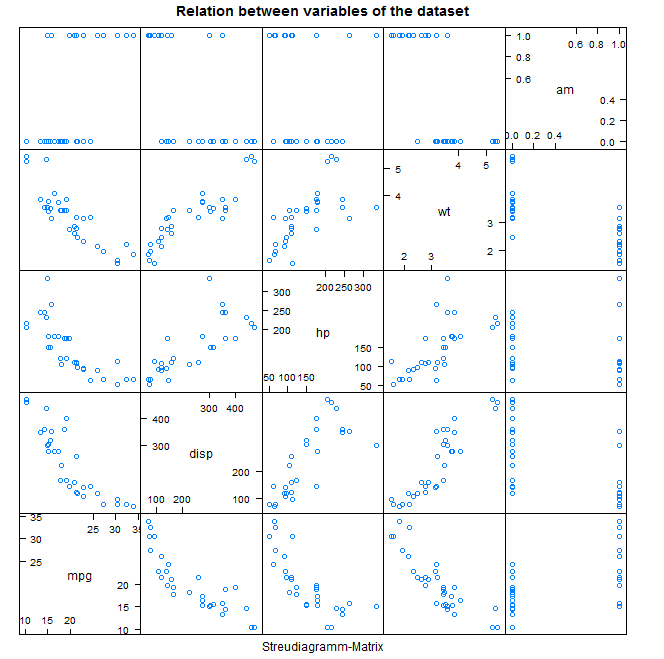
\includegraphics[width=1.0\linewidth]{scatterplot_matrix}
\caption{Scatterplot Matrix}
\end{figure}

\newpage
\section{Residuals}

The residuals for the model were examined. The following four methods were utilized in order to determine the goodness of fit.

\begin{itemize}
 \item Residuals vs Fitted
 \item QQ-Plot to examine normal distribution of residuals
 \item Standarized residuals
 \item Residuals vs Leverage
\end{itemize}

\begin{figure}
\centering
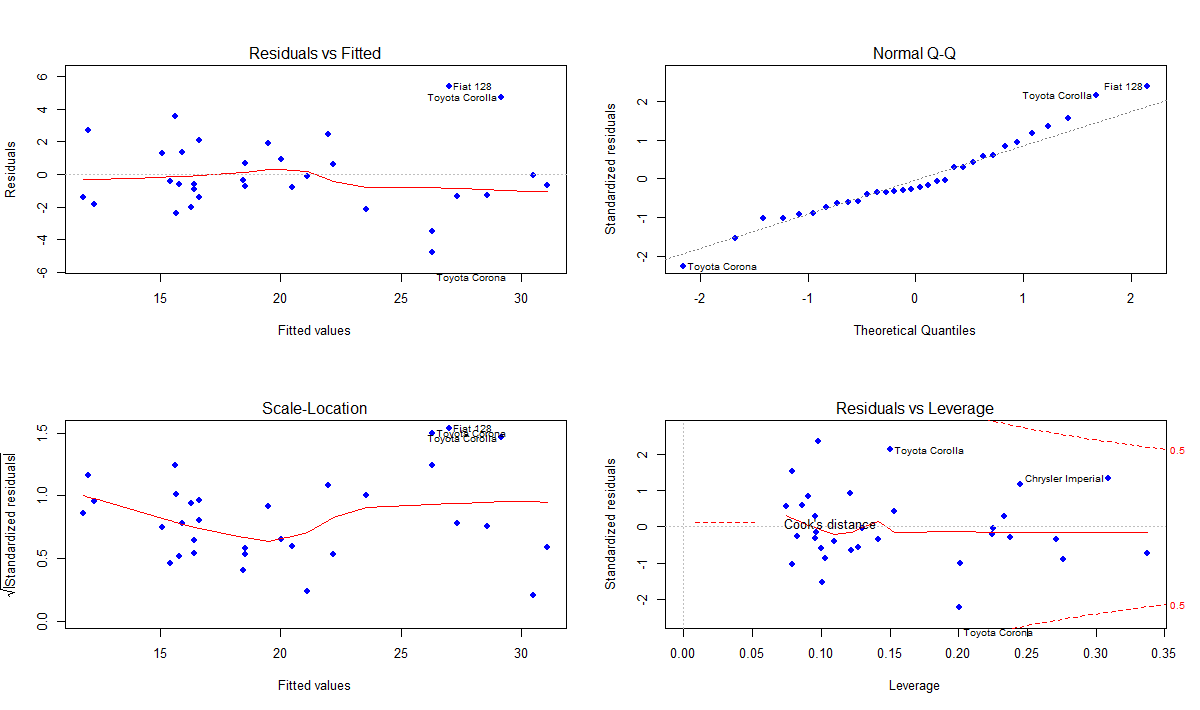
\includegraphics[width=1.2\linewidth]{residuals}
\caption[Residuals]{Residuals}
\end{figure}

Residuals are in a good approximation normally distributed. No autocorrelation nor heteroskedasticity could be observed.
However, two car models - the Toyota Corolla and the Fiat 128 - show greater residuals tha expectetd. This might be due to the fact that these small cars were engineered to save gasoline, opposite to the majority of the investigated population.

\end{document}